\section{Signatures and Observables}
\label{s_signatures}


% TODO: ADD REFERENCES FOR THE TABLE INFORMATION

Figure \ref{fig:signatures} is a table-in-progress to identify potential signatures and observables of illicit activity at all major facilities in the nuclear fuel cycle.  Each potential signature is color coded to represent the accessibility of the data.  Green signatures are available through open, independent sources such as satellite imagery.  Blue signatures may not be publicly available but could be attained through official channels such as IAEA inspections.  Yellow signatures may or may not be made available but must be considered unreliable or unverifiable due to physical or political constraints, e.g. state declarations.  Not all of these signatures are currently collected, and it would be resource intensive to maintain comprehensive surveillance of all signatures.  For example, a truck that leaves a fuel fabrication plant should arrive at a reactor (or train station) with the fuel shipment, but it is infeasible to comprehensively track individual truck movement.  However, correlations in these individual signatures can be leveraged to overcome sparse datasets or resource constraints.


% TODO: REMOVE RED BOXES or add to legend, REMOVE purple boxes. Clean up further if needed? 
% Google spreadsheet: CVT_Research/Collaborations/Fuel Cycle Facility Signatures
\begin{figure}%[htbp!]
\begin{center}
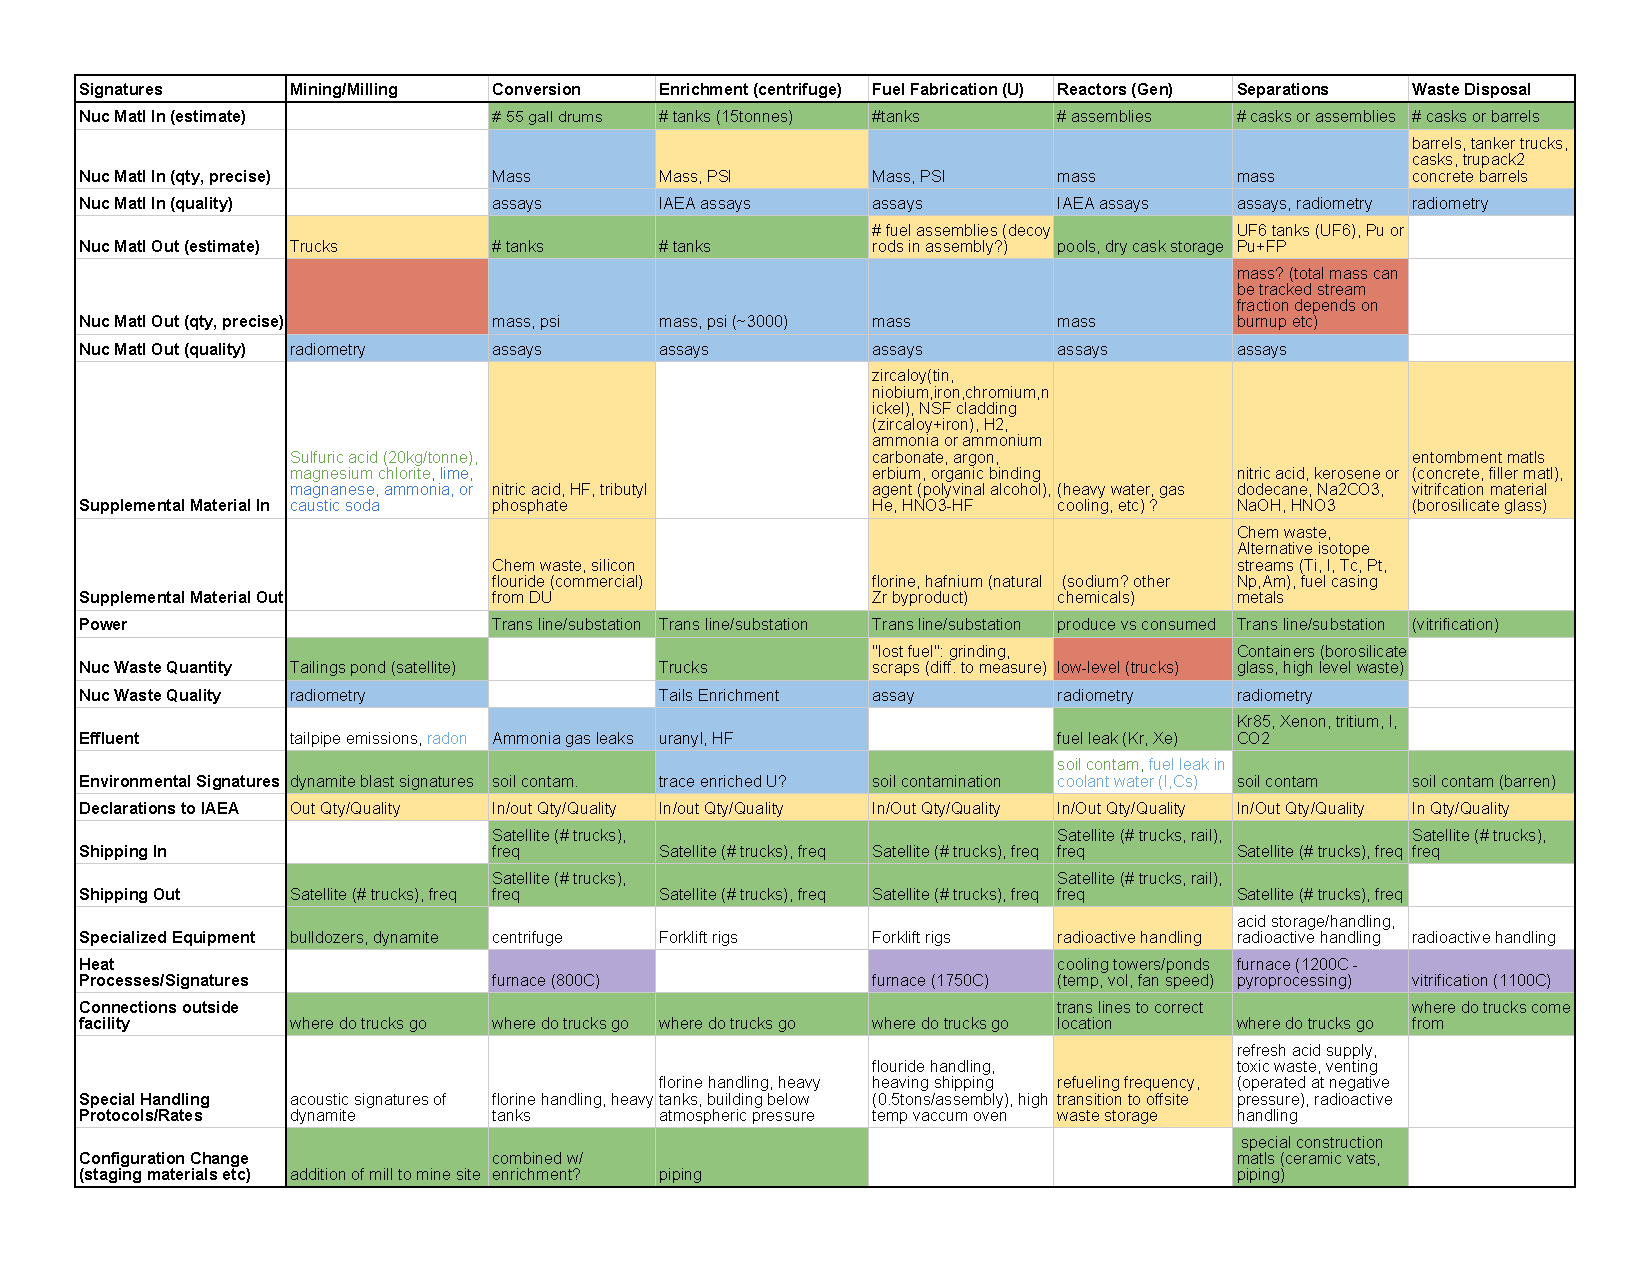
\includegraphics[natwidth=162bp,natheight=227bp, scale=0.6]{./figs/signatures_table.pdf}
\end{center}
\caption{Table of potential signatures across the fuel cycle. Green=measureable through open, independent sources such as satellite imagery, Blue=available through official inspections, Yellow=data may be unreliable due to physical or political constraints.}
\label{fig:signatures}
\end{figure}

\Cyclus is being used to produce a variety of synthetic signals spanning a range of modalities.  We are currently developing signatures that would be available either publicly or via official inspections (green or blue).  As can be seen in Section \ref{s_results}, all facilities in \Cyclus automatically produce time-series data of material inventory.  Additionally, the enrichment facility reports it's SWU consumption as a time series that can be used as a rough proxy for facility power consumption. As seen in Figure \ref{fig:effluent}, \Cyclus can combine atmospheric transport models with facility effluent concentration ($I$) to track geographic dispersion. In this example, a simple atmospheric diffusion model of wind from the left is used to illustrate how a clandestine reprocessing facility (middle) could be hidden in close proximity to two declared facilities (top and bottom)\cite{simple_transport_model}.  In addition to regularly sampled time-series data, \Cyclus also models sparse, discrete-event data such as declared truck shipments from a facility.


% /Users/mbmcgarry/git/data_analysis/data/v1.3/pu_reprocess/
\begin{figure}%[htbp!]
\begin{center}
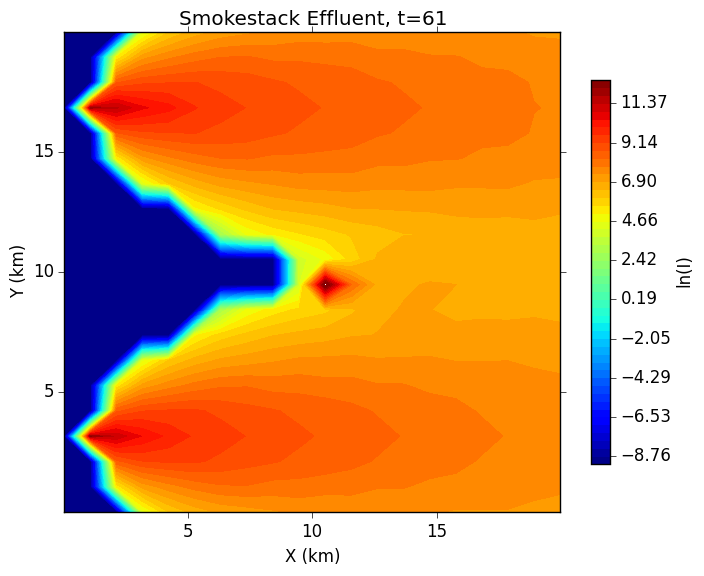
\includegraphics[natwidth=162bp,natheight=227bp, scale=0.6]{./figs/proper_diff_fr61.png}
\end{center}
\caption{Effluent transport with wind from left, hides a clandestine reprocessing facility (x,y)=(11,9) in close proximity to two declared facilities ((x,y)=(1,3), (1,17)}
\label{fig:signatures}
\end{figure}

\Cyclus is also being used to model inspections at an enrichment facility that test for the presence of \gls{HEU}. IAEA inspections typically involve multiple swipe samples per location, with some likelihood of false-positive or false-negative results.\cite{INSPECTION_FALSE?}.  Figure \ref{fig:inspect} pairs inspections with undeclared truck shipments of \gls{HEU}. In this example, it is assumed that the likelihood of detecting \gls{HEU} in the enrichment facility increases with each shipment (because contamination is possible when \gls{HEU} is removed from cascades and bottled for shipping).  The undeclared \gls{HEU} shipments are shown as black bars, where amplitude incorporates the gross quantity \gls{HEU} that has been produced at the facility. The colored dots scale from yellow to red, indicating the fraction of positive swipes at an \gls{IAEA} inspector visit (assumiing a total of 10 swipes are taken per inspection, and an average of two inspections per year).  It is assumed that both false-positive and false-negative results are possible. 

% /Users/mbmcgarry/git/data_analysis/data/UM_data/multi_modal_v1.3/single_runs/inspect_example
\begin{figure}%[htbp!]
\begin{center}
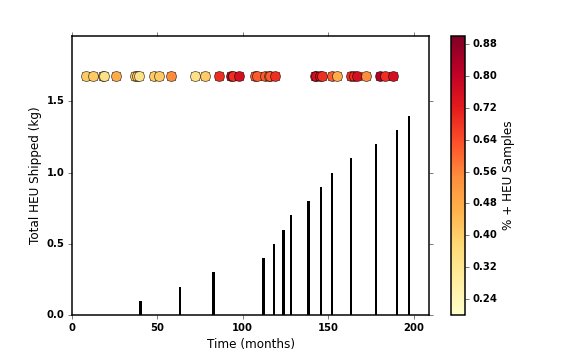
\includegraphics[natwidth=162bp,natheight=227bp, scale=0.6]{./figs/mm_5enr_lowtails_insp_200yrinspect_ship.png}
\end{center}
\caption{Black bars indicate clandestine shipments of \gls{HEU}, amplitudes show gross \gls{HEU} production at the enrichment facility.  Colored circles are fraction of swipes (out of 10) testing positive for \gls{HEU} during an inspection. Both false positives and false negatives may be present, introducing uncertainty into the data. As more \gls{HEU} is produced, the detection rate increases.}
\label{fig:signatures}
\end{figure}

Figure \fig{false_inspect} shows the breakdown of true positive, false positive, and false negative results for each inspection (for illustrative purposes only, in practice the true accuracy of a particular set of field data is unknowable).  Before month 30, no \gls{HEU} has been produced in the facility, so any ``positive'' swipes are false-positives (tan). Once the facility begins producing \gls{HEU}, liklihood of contamination increases until it is detected near month 80. If the swipe tests were perfect, there would be a 100\% detection rate for all inspections after that time. However, the possibility of false-negatives (pink), make it so that the measured inspection data appears to be the tan before month 80 and the red after month 80.  In this scenario, it would be difficult for an inspector to conclude that \gls{HEU} was being produced with this dataset alone.

\begin{figure}%[htbp!]
\begin{center}
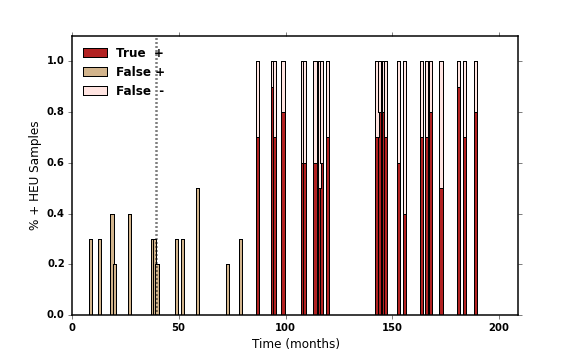
\includegraphics[natwidth=162bp,natheight=227bp, scale=0.6]{./figs/mm_5enr_lowtails_insp_200yrswipe_rates.png}
\end{center}
\caption{The scenario in Figure \ref{fig:signatures} had a 30\% rate for both false-positives and false-negatives. Before month 30, no HEU has been produced so all detections are false positives (tan). Once \gls{HEU} contamination is present (near month 80), true detections (red) combine with false-negatives (pink), resulting in a effective 70\% detection rate.}
\label{fig:signatures}
\end{figure}
